\documentclass[11pt]{article}
\usepackage[a4paper,margin=0.85in]{geometry}
\usepackage{graphicx}
\usepackage{booktabs}
\usepackage{enumitem}
\usepackage{amsmath}
\usepackage[hidelinks]{hyperref}

\title{\textbf{NeuralFabric: Technical Project Explanation}}
\author{Divyank Seervi \and Choppa Madhu Dhanush Teja \and Krish \and Srishti Agarwal\\\textit{SCOPE, VIT Vellore}}
\date{}

\begin{document}
\maketitle

\section*{1. Problem Statement}
Datacenter applications can generate bursty traffic. A simple multipath policy such as ECMP distributes flows across equal-cost paths, but it does not directly predict how the queue state will evolve. When several flows become concentrated on the same links, queues can grow and packets can be dropped.

NeuralFabric studies whether recent telemetry can be used to forecast future link congestion and whether a controller can act on that forecast without causing excessive route changes.

\textbf{Important scope:} this project is a synthetic research prototype. It does not implement a production Ethernet switch, RoCEv2, PFC, ECN, DCQCN, NCCL, or a real-time control plane. Its purpose is to test an algorithmic hypothesis in a controlled simulator.

\section*{2. Overall Pipeline}
The project contains five main stages:
\begin{enumerate}[leftmargin=*]
    \item \textbf{Traffic generation:} six synthetic traffic families create flows on a k=4 Fat-Tree.
    \item \textbf{Network simulation:} a causal FIFO packet-batch engine advances packets one link per 1 ms tick.
    \item \textbf{Telemetry extraction:} node and switch-to-switch link statistics are converted into normalized feature vectors.
    \item \textbf{Congestion prediction:} a GCN-LSTM receives a ten-tick history and predicts a link-level congestion score five ticks after the last observed feature.
    \item \textbf{Routing admission:} the guarded controller considers route changes only when predicted risk, path quality, capacity, freshness, cooldown, and change-budget rules are satisfied.
\end{enumerate}

\begin{figure}[h]
\centering
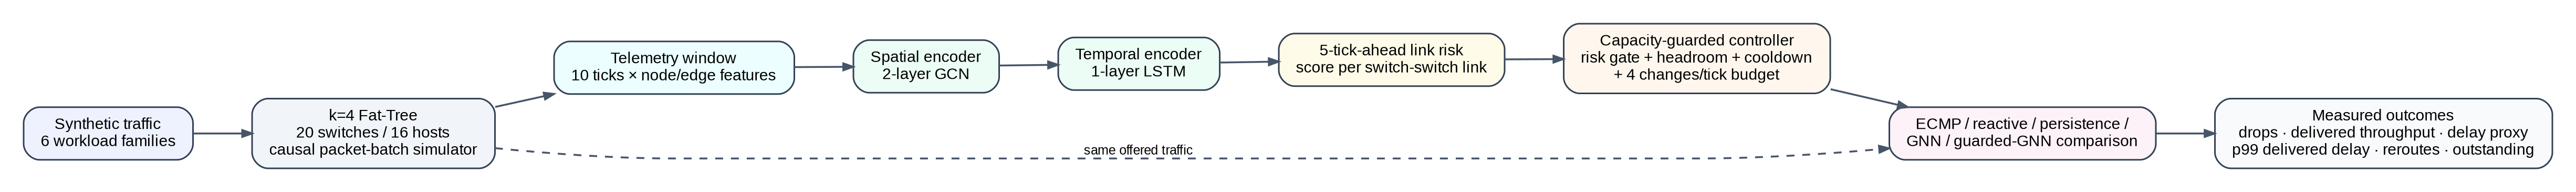
\includegraphics[width=0.94\textwidth]{research/system_architecture.png}
\caption{Implementation pipeline used by the project.}
\end{figure}

\section*{3. Network Simulator}
The default topology contains 20 switches, 16 hosts, 32 switch-to-switch links, and 48 physical links. Each physical link uses one shared FIFO queue for both directions. The configured simulated capacity is 500 packets/tick, the buffer limit is 2000 packets, and the time step is 1 ms. A nominal 10 Gbps field is retained as topology metadata and is not converted into the packet capacity.

At every tick, active flows generate packets, packets enter the first hop, each FIFO serves up to its capacity, and departures either move to the next hop on the following tick or become delivered packets at the destination. Queue-full packets are counted as drops. The simulator verifies:
\[
P_{offered}=P_{dropped}+P_{delivered}+P_{outstanding}.
\]

This accounting check is important because a simulator can otherwise create misleading routing improvements by duplicating, deleting, or double-counting traffic.

\section*{4. What the Model Learns}
Each switch has four normalized node features:
\begin{center}
queue occupancy, throughput, drops, and buffer usage.
\end{center}
Each switch-to-switch link has four edge features:
\begin{center}
offered utilization, queue depth, drop rate, and latency proxy.
\end{center}

The congestion label is 1 when raw offered arrivals on a link exceed 85\% of the configured packet capacity. The model receives the previous ten ticks and predicts this future label five ticks after the last observed feature.

\section*{5. GCN-LSTM Model}
The model has two spatial and one temporal component.

\textbf{GCN:} a graph convolution layer lets each switch representation incorporate information from neighboring switches. Two GCN layers are used, with layer normalization, ReLU, and dropout.

\textbf{Edge embedding:} for every switch-to-switch link, the source embedding, destination embedding, and link features are concatenated and projected to 32 dimensions.

\textbf{LSTM:} a one-layer LSTM processes each link's 10-tick history and provides a temporal representation.

\textbf{Prediction head:} a small multilayer perceptron maps the LSTM representation to a sigmoid congestion score.

The final implementation contains 17,985 trainable parameters.

\section*{6. Why Persistence Is a Necessary Baseline}
A neural model can look good simply because the underlying network state changes slowly. Therefore the project includes a persistence baseline: it predicts that the last observed congestion label will remain unchanged.

The recorded held-out results are:
\begin{center}
\begin{tabular}{lrrrr}
\toprule
Predictor & F1 & AP & ROC AUC & Brier\\
\midrule
GCN-LSTM & 0.7940 & 0.8692 & 0.9580 & 0.0676\\
Persistence & 0.8118 & 0.6991 & 0.8799 & 0.0777\\
\bottomrule
\end{tabular}
\end{center}

This result should be explained honestly: the GCN-LSTM has better ranking and Brier metrics but lower F1 at the fixed 0.5 cutoff. Therefore the experiments do not prove that the neural predictor is always necessary.

\section*{7. Capacity-Guarded Controller}
The controller is the main algorithmic component of the project. It uses a forecast score for every switch-to-switch edge and computes a path risk as the maximum predicted risk on that path:
\[
r(\pi)=\max_{e\in\pi} p_e.
\]

A flow becomes a candidate for rerouting when its current path risk exceeds 0.7. A new path is accepted only if:
\begin{itemize}[leftmargin=*]
    \item predicted path risk improves by at least 0.15;
    \item path length increases by no more than two hops;
    \item the prediction is not stale by more than one tick;
    \item the flow is outside its five-tick reroute cooldown;
    \item the controller has not exceeded four changes in the current tick; and
    \item every newly added link passes the capacity-reservation check.
\end{itemize}

For a newly added link $e$, the guard checks:
\[
D(e)+r_f+Q(e)\leq0.90C(e),
\]
where $D(e)$ is the conservative current demand estimate, $r_f$ is the moved flow rate, $Q(e)$ is queued traffic, and $C(e)$ is configured capacity.

The important idea is sequential reservation: after a route is accepted, its demand is added to the new links before another route decision is made. Therefore multiple flows cannot all assume that the same headroom is still available.

\section*{8. Experimental Design}
The recorded research experiment uses 30 data scenarios for model development. Whole scenarios are assigned to train, validation, and test groups (21/4/5), preventing overlapping windows from being split across partitions.

For routing, six traffic families are evaluated using three independent seeds per family. Five strategies are compared on each matched seed:
\begin{center}
ECMP, Reactive, Persistence, GNN, Guarded GNN.
\end{center}
This produces 6 $\times$ 3 $\times$ 5 = 90 routing runs.

\section*{9. Main Results}
The strongest recorded workload-specific result is the stride workload:
\begin{center}
\textbf{59,840 drops (ECMP) $\rightarrow$ 8,113 drops (Guarded GNN), an 86.4\% reduction.}
\end{center}

Across all 18 matched traffic trials, the guarded controller has:
\begin{center}
\begin{tabular}{lrr}
\toprule
Metric & ECMP & Guarded GNN\\
\midrule
Mean drops/run & 301,821.5 & 283,899.0\\
Mean delivered packets/tick & 1,852.28 & 1,979.47\\
Mean delivered delay & 9.664 ms & 9.008 ms\\
Mean run p99 delay & 17.389 ms & 15.889 ms\\
Mean reroutes/run & 0.00 & 14.72\\
\bottomrule
\end{tabular}
\end{center}

The guarded controller beats or ties ECMP in all 18 matched trials: 15 wins, 3 ties, 0 losses. Its average drop reduction is 5.94\% against ECMP. Reactive rerouting averages 622.83 route mutations per run, while Guarded GNN averages 14.72, a 97.6\% reduction in route mutations.

\begin{figure}[h]
\centering
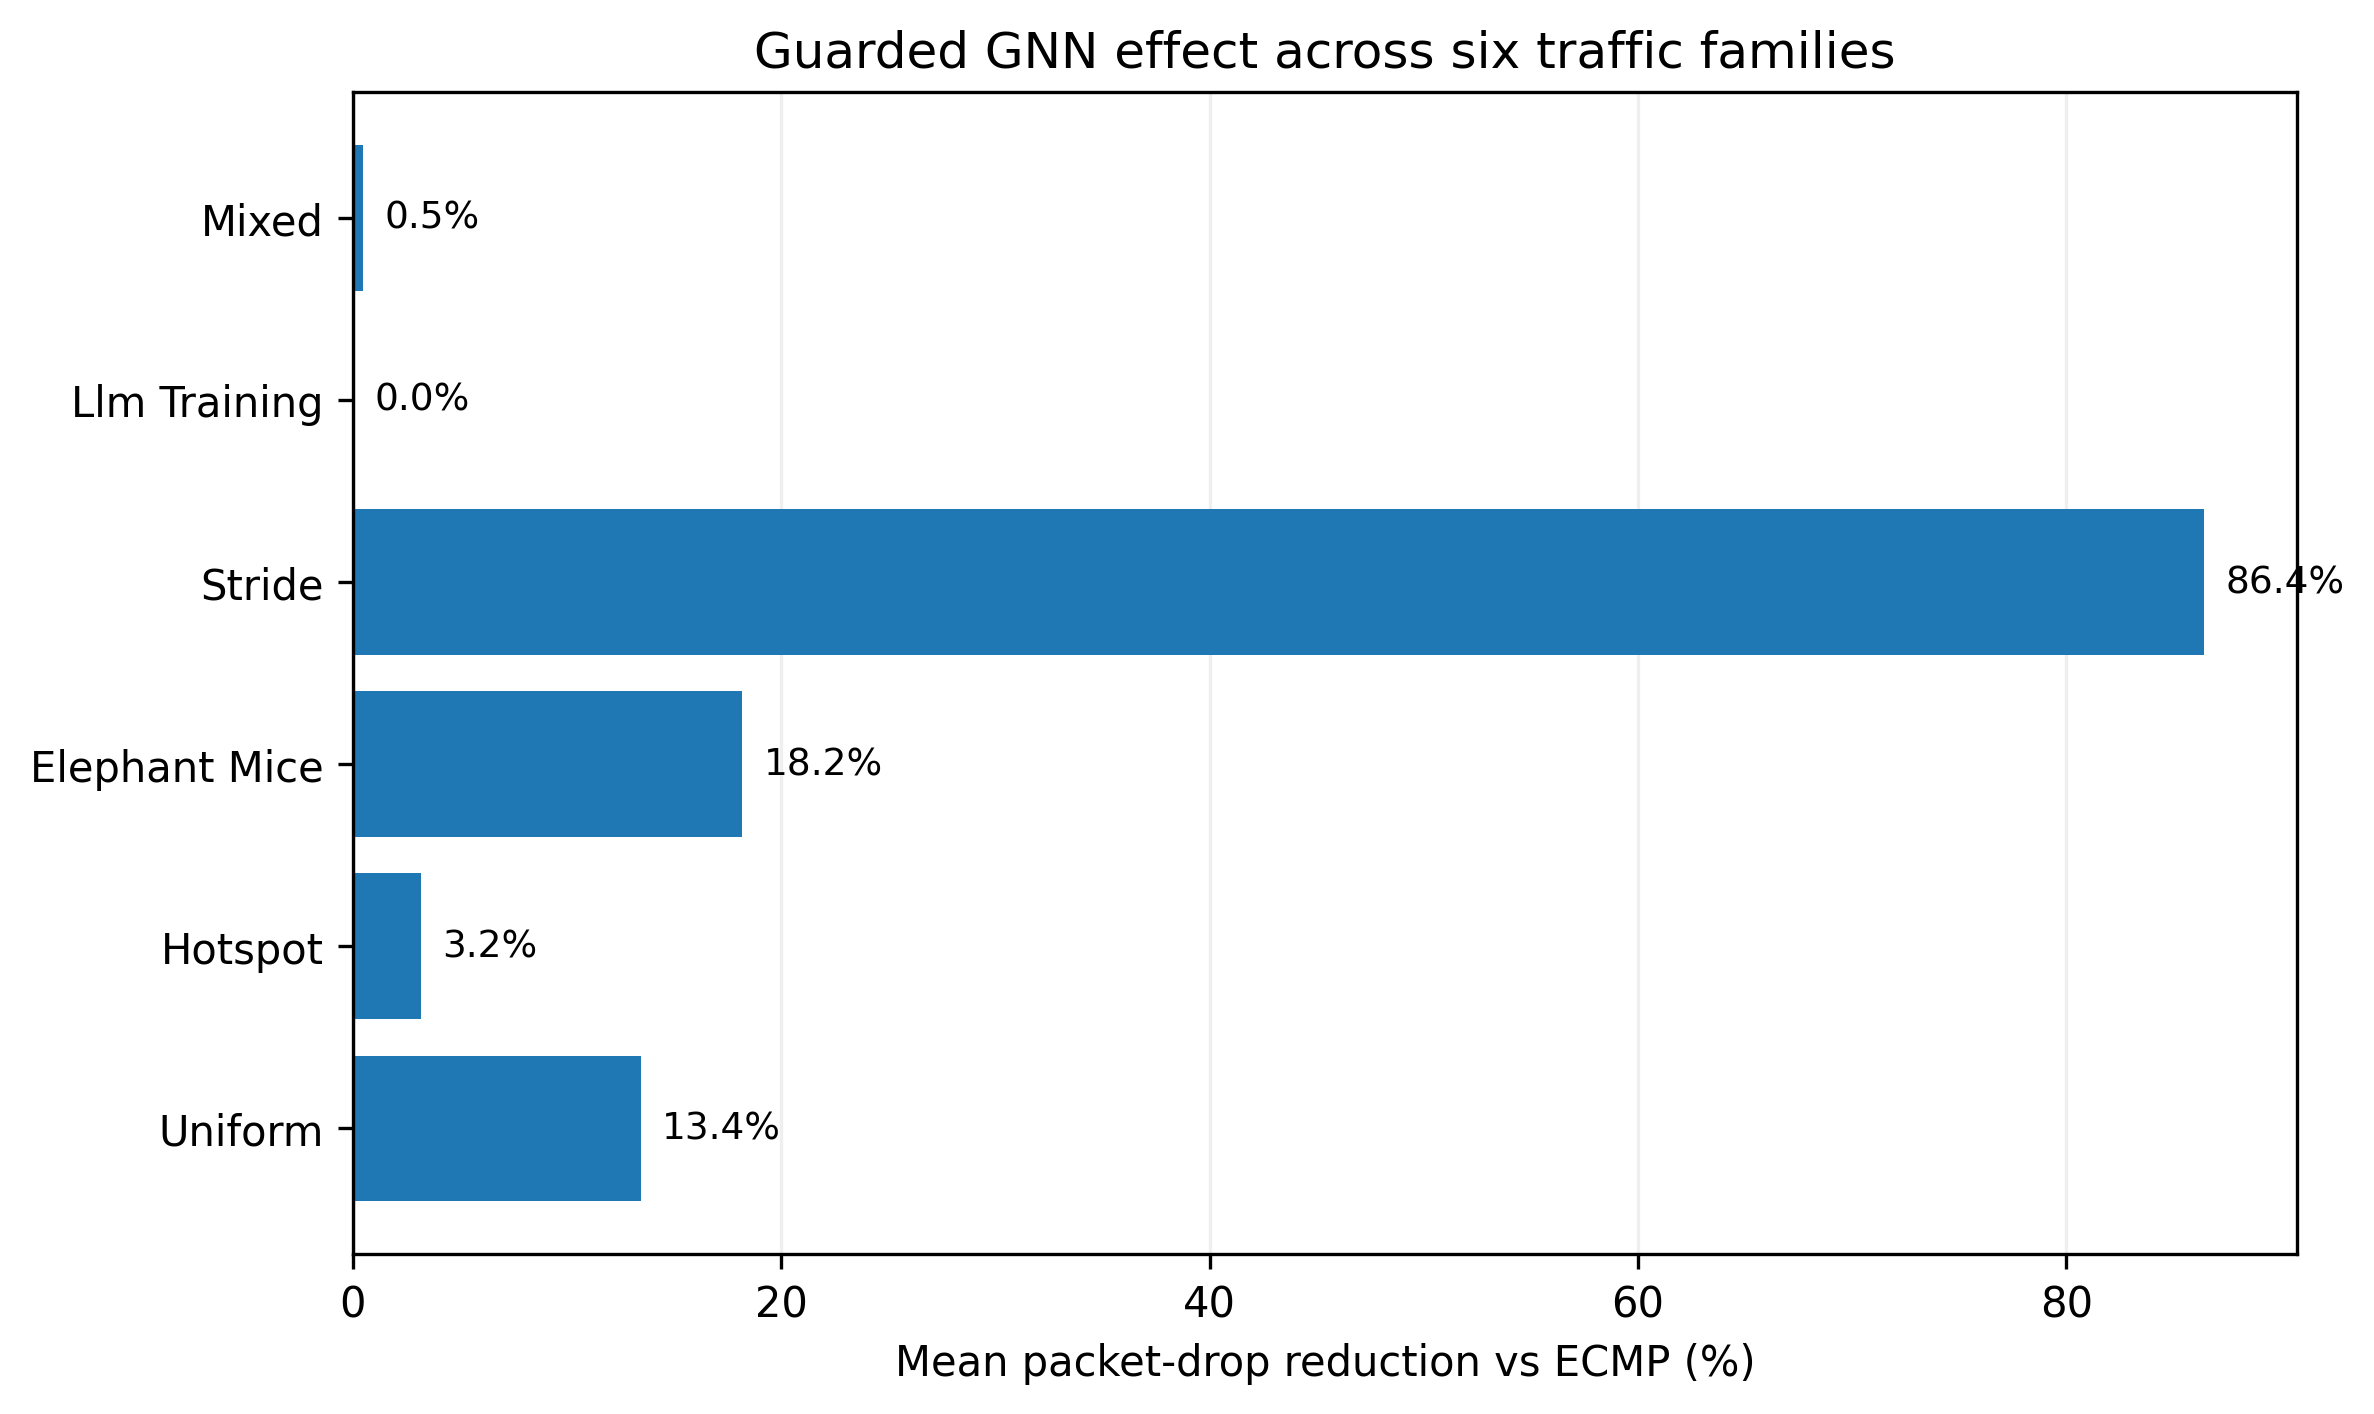
\includegraphics[width=0.94\textwidth]{research/drop_reduction.png}
\caption{Guarded GNN drop reduction relative to ECMP across the six traffic families.}
\end{figure}

\section*{10. How to Interpret the Results}
The project should not be presented as ``the GNN always predicts better'' or ``the controller solves datacenter congestion.'' The measured evidence supports a narrower statement:

\begin{quote}
In this synthetic simulator, adding explicit capacity and stability guards to a forecast-driven rerouting policy improves routing outcomes over stable ECMP on the recorded workloads while greatly reducing route mutations compared with an unconstrained reactive controller.
\end{quote}

The strongest improvement occurs in structured stride traffic. Hotspot traffic is harder because routing may not remove a destination-side bottleneck. The mixed workload produces only a 0.49\% reduction relative to ECMP. These differences are important and should remain visible in the presentation.

\section*{11. What the Project Does Not Claim}
\begin{itemize}[leftmargin=*]
    \item It does not prove microsecond response time. The simulator tick is 1 ms.
    \item It does not simulate or prevent PFC deadlocks.
    \item It does not model RoCEv2 transport, packet ordering, retransmission, or NIC behavior.
    \item It does not execute real GPU/NCCL training traffic.
    \item It does not measure a switch-programming or controller-network delay.
    \item It does not establish production readiness or patentability.
\end{itemize}

The recorded host inference p99 is 6.185--13.516 ms, and some tails therefore exceed the 5 ms forecast horizon. That is a limitation of the current prototype, not a result to hide.

\section*{12. Reproducibility}
The project includes:
\begin{itemize}[leftmargin=*]
    \item the source code for simulation, telemetry, model training, routing, and dashboard execution;
    \item the recorded dataset and trained checkpoint;
    \item 13 regression/integration tests;
    \item the raw structured benchmark in \texttt{research/benchmark\_results.json};
    \item a tested dependency file in \texttt{requirements-tested.txt}; and
    \item scripts for rebuilding the experiment and visualizations.
\end{itemize}

Run the tests before a demonstration. The dashboard can then be launched locally to visualize the topology, telemetry, predictions, and guarded route changes.

\section*{13. Final Takeaway for a Viva}
A good one-line explanation is:

\textbf{``NeuralFabric forecasts which links are likely to become congested and lets a routing controller move flows only when the alternative path passes explicit capacity and stability checks.''}

The important engineering lesson is that prediction alone is not enough. A forecast-driven controller needs safeguards because an incorrect or simultaneous routing decision can create a new bottleneck. The project demonstrates that principle in a controlled synthetic environment and identifies the experiments required before the idea can be evaluated on a real datacenter network.

\end{document}
